\chapter{The Pineapple Leaves Route}
\label{FLPchapt4}

As discussed in \cref{chapter_3lab}, although small-scale projects of Pineapple Leaves (PAL) valorisation have been conducted, it is not clear how an industrial-scale valorisation process would be carried out operationally. Minimising costs in the valorisation process is paramount should PAL-based products compete with conventional, fossil-fuel-based products. The process of valorising PAL can be divided into three main stages: extraction, transportation, and material transformation. In this chapter, we focus on the last two by developing a Facility Location Problem in which we try to locate and minimise the optimal number of material transformation facilities conditional on the location of pineapple fields in Costa Rica, the costs of transporting biomass (PAL), and the costs of opening and operating a hypothetical PAL valorisation facility.

\section{Facility Location Problem}
\label{FLPlit}

The Facility Location Problem (FLP) is an optimisation problem that determines the best location for the facilities to be placed based on the costs of the facility, geographic demands and transportation distances. The results drawn from an FLP are critical in strategic planning for private and public entities. Due to the high costs of property acquisition and facility construction, facility location decisions are long-term strategic investments. FLP became relevant due to the industrial revolution, as the development of rail transport, energy, and urban growth offered more options to distribute firms and their operations. Alfred Weber first developed a theory of location problems with his publication \textit{Über den Standort der Industrie} (Theory of the Location of Industries) in 1909, in which he modelled an optimal location and minimal cost for manufacturing plants taking into account several spatial factors \citep{fearon2006alfred}. Since the 1960s, when \citeauthor{hakimi1964optimum} published his work on an FLP for switching centres in a communication network and police stations in a highway system, there have been numerous studies on different types of FLP \citep{farahani2009facility}.

Location problems consist of four main components: existing demand points, some facilities that are supposed to serve the demand points, a feasible solution space in which the demand points and facilities are dispersed, and a measurement criterion that explains distances (e.g., time or cost) between facilities. Although there are many versions of the FLP applied to different types of problem, they are all comprised of an objective function and a set of constraints. The many ways in which FLP can be categorised are explained by \cite{wolf2022solving}. First, we can consider private- and public-sector location problems. In the former, the objective functions are profit maximisation or cost minimisation, while the public sector problems also consider nonmonetary costs and benefits, such as environmental costs when locating hazardous waste repositories or the value of saved lives when establishing emergency centres. 

The second classification is planar versus network location problems: In planar FLP, the locations of a finite number of demand points and of the optimal facilities may be dispersed everywhere in the Euclidean plane. On the contrary, network location problems are defined on networks composed of nodes and edges. Almost all network location problems assume that the demand and facility points coincide with the vertices of a network and that transport occurs only along the edges of this network. The weights assigned to the edges can specify not only distances but also travel times or transportation cost. These terms might remind us of \cref{chapter_3lab}, in which we modelled a Fuzzy Cognitive Map (FCM) composed of concepts (nodes) that affect each other through the weighted edges of a network. In the FLP, we study a different problem, but it is still interesting to highlight how graph theory is used in a wide range of applications \citep{papageorgiou2003fuzzy, seppanen1970facilities}. Both planar and network FLP can be continuous, meaning that the generation of feasible sites is left to the model at hand, or discrete space problems, in which facility candidates are selected a priori. Even when problems are continuous by nature, most of the results in the literature are discretised.

FLP can also be categorised into capacitated or uncapacitated problems. Capacitated facilities have a constrained capacity to serve demand sites, while uncapacitated facilities are unrestricted. A fourth relevant classification of FLP is when we consider solving for desirable or undesirable facilities. Most problems locate desirable facilities, such as warehouses, service centres, or hospitals as close as possible to the demand points. On the contrary, when dealing with undesirable facilities, such as landfills, polluting plants, etc., the objective function of the FLP is to maximise the weighted distance function between the facilities and the served demand points. Finally, we consider the classification of FLP by the number of facilities to be located. When the number of facilities is specified exogenously, the problem can be either single or multi-facility. On the contrary, FLP can also be defined with an output parameter of the number of facilities to be optimised. It is important to note that the number of facilities influences the execution time of any algorithm. In complexity theory, the general problem of locating optimal facilities in a network is NP-hard. NP, which stands for non-deterministic polynomial, is a set of problems whose solutions can be verified in polynomial time. Yet, it is unknown whether NP-hard problems have an algorithm for finding the solution in polynomial time; this question is known as the P versus NP problem. NP-hard problems are at least as hard as the hardest problems in NP and are considered to be some of the most difficult problems to solve using algorithms \cite{kokash2005introduction, cooper1963location}.

In operations research, as well as in other fields, optimisation problems are defined as NP-hard problems. A few decades ago, only problems small enough (e.g., \cite{sridharan1995capacitated} indicate 50 facilities and 50 demand points) could be handled using exact mathematical methods. Thus, researchers came up with heuristic and metaheuristic methods, which are approximation methods that can find a good enough solution in a reasonable time. Heuristic methods are usually defined for the particular problem it seeks to solve and can become insufficient for other problems. Metaheuristic methods, on the contrary, are generic, problem-independent algorithms that can be adapted to almost all optimisation problems. Exact methods find the optimal solution, but they can be computationally intensive and impractical for large problems. (Meta)heuristic methods, on the other hand, overcome the NP-hardness of the optimisation problems by finding a good enough solution quickly and efficiently but may not guarantee an optimal solution. The most common metaheuristic methods are simulated annealing, tabu search, genetic algorithm, variable neighbourhood search, and ant systems. All of these are designed to decrease the probability of falling in local optimal \citep{abdel2018metaheuristic}. Optimisation solvers and hardware have become much faster in the last two decades, and now it is less common to require complicated (meta)heuristic models \cite{gurobiFast}.

The use of FLP for waste management and waste valorisation and biomass conversion is common in the literature. The linear economy and the throwaway culture led to an increase in waste generation. Consequently, the disposal of waste has become a relevant problem throughout the world. Operations research provides the tools needed to optimise waste disposal and minimise the costs and environmental degradation caused by waste management. \cite{adeleke2020facility} provides a good summary of the existing FLP models and optimisation techniques and their application to solid waste management problems. Most studies focus on the treatment of municipal, industrial, healthcare, and hazardous waste. As waste can have more than one disposal site, it is important to consider other facilities associated with collection sites, such as recycling centres and landfills. This also applies when implementing residue valorisation processes.\cite{hu2017bi} developed a facility location model that minimises government spending and environmental adverse effects in the location of waste-to-energy facilities. Another good example of an FLP that takes environmental costs into account is the study of waste collection in China by \cite{wu2020optimization}, which considers greenhouse gas emission costs and conventional waste management costs. \cite{athira2020effective} used a location-allocation analysis to optimise the location of new cement plants based on the availability of sugarcane bagasse ash produced in the sugar industry, which can serve as a supplementary and partial alternative to cementitious material. \cite{guerrero2016gis} assessed the use of banana crop residues in the generation of bioethanol and identified two optimal locations for energy conversion facilities in Ecuador, a major banana producer country. Another example of a biorefinery location optimisation is the study by \cite{duarte2014facility}, who applied a mixed-integer linear programming formulation to locate a second-generation bioethanol plant fed with coffee cut stems in Colombia. \cite{nordin2022optimal} conducted a study of the cost-effective localisation of ethanol production facilities in Sweden and concluded that feedstock costs are the most important factor in determining location, followed by high feedstock density. More importantly, at higher production, feedstock from the whole country is preferred despite high transport costs. A complex multi-objective optimisation model was developed taking into account financial costs and CO2 emissions \cite{harris2014hybrid}. Here we comment on relevant studies for the following discussion, but there are many more examples of different types of FLP applied to waste management and valorisation solutions \citep{bojic2018location, harris2009multi, kocoloski2011impacts, wetterlund2012optimal}.

\section{Case study description}

Following the different types of categorisation described above, we describe the present FLP as a private sector, network-dependent, capacitated, desirable, and multi-facility problem. We apply a simple Capacitated Plant Location Problem (CPLP) with a single echelon (one distribution network level) to a scenario of PAL-based biogas production in Costa Rica. As described in \cref{neweconomy}, the pineapple crop residues can be used to produce several biobased materials and second-generation biofuels. Because none of the described processes has been implemented on a large scale, there is no information on the production capacity and costs of a candidate processing facility. Thus, we use estimates based on previous experiments from Costa Rica and data from similar cases. We chose biogas plants as the example solution for several reasons. Data on the costs and production capacity of biogas plants are easily accessible, but data on biobased materials are scarce. Nonetheless, to recycle all the PAL, a combination of various valorisation processes will be necessary. In this sense, our study can be expanded to include complementary processes once we have collected more data.

The production of bioethanol is perhaps the most effective solution to minimise residues and process large amounts of PAL, but the costs associated with opening and operating a biorefinery for bioethanol production require large investments, which can only be plausible in a scenario of high cooperation between stakeholders or involvement of the government. As discussed in \cref{chapter_3lab}, such a scenario is not present today. The technology of biogas plants is well developed, and their capacities allow for larger amounts of PAL than other solutions, making their investment cost-effective for a pineapple producer. It should be noted that the scenario described here is based on the available technology and the current situation of the social dynamic of the pineapple sector in Costa Rica. Should more efficient solutions become available, including multi-product solutions, the FLP modelled in this study can be adjusted to generate new optimal solutions. 

Let us now describe the study area in Costa Rica. The United Nations Development Programme (UNDP), the Ministry of Environment and Energy (MINAE), and the National Centre for Geoenvironmental Information (CENIGA) carry out a monitoring of the changes in pineapple crops and their consequences on forest cover using satellite data. They indicate that the average accuracy of the layers is 99.5\%. The latest available data is for 2019 \cite{SNITpina}. We use the data collected by these organisations to determine the location and amount of available PAL in the country.

In \cref{allCRPAL}, the 65,451 hectares of pineapple crops in Costa Rica as of 2019 are depicted. 870 hectares (1.32\% of the total) are located in the west of the country, specifically in Judas, Puntarenas province. 8072 hectares (12.33\% of the total) are clustered in the south, between Potrero Grande and San Isidro de El General. The remaining 56,509 (86\% of the total) of pineapple hectares are located in the northeast of the country, in the regions Huetar Norte and Huetar Caribe. Including crops located in the south and west of the country would hinder the FLP analysis as the area in which the candidate location can be located would be much larger. Since the percentage of PAL in those regions is not large, we narrow the selection and carry out the analysis for the crops located in the north-east of Costa Rica, specifically in the bounding box -85.07, -81.5, 10.09, 11.04 (west, east, south, north). 


\begin{figure}[H]
\caption[Pineapple crops in Costa Rica]{Pineapple crops in Costa Rica. The crops in the northeast are coloured green and the crops in the west and south are coloured blue.}  
\label{allCRPAL}
\centering
\includegraphics[width=\textwidth]{fig/allCostaRicaPAL.pdf}
\end{figure}


\section{Model description}

The CPLP, as described in \cite{farahani2009facility}, is formulated as a mixed-integer linear programming model of the following form:

\begin{equation}
\label{objectivefun}
    \text{Min} \sum_{i \in U} \sum_{j \in V} c_{ij} \ x_{ij} + \sum f_i \ y_i,
\end{equation} 

subject to:
\begin{gather}
    \label{capacity}
    \sum_{j \in V} d_{j} \ x_{ij} \leq q_{i} \ y_{i} \\ 
    \label{onetone}
    x_{ij}\geq 0 \\
    y_i \in \{0,1\},
\end{gather}

where:
\begin{description}

    \item U: The set of potential facilities,
    
    \item V: The set of PAL source points (pineapple fields),
    
    \item $d_j$: The PAL supply of the farm $j$,
    
    \item $q_i$: The capacity of the facility $i$,
    
    \item $c_{ij}$: The cost of transporting all the PAL supply from the farm $j$ to the facility $i$, 
    
    \item $f_i$: The fixed cost associated with opening the facility $i$,
    
    \item $y_i$: A binary decision variable that takes the value 1 if the facility $i$ is open and 0 otherwise,
    
    \item $x_{ij}$: A continuous decision variable, corresponding to the fraction of the PAL supply $j$ absorbed by the facility $i$.
    
\end{description}

The objective function attempts to minimise the total cost of opening and operating a processing facility. This is described in \cref{objectivefun} as the sum of the cost of opening the facilities and the cost related to processing the supply of PAL. \cref{capacity} states that no farm can ship to a closed facility and that the total PAL supplied from each farm does not exceed the capacity of the facility. Ultimately, the total cost measures the trade-off between the cost of building a new facility and the total cost of transportation.  


\section{Material}

\subsection{Source of PAL}

Pineapple crops in Costa Rica are harvested on average every two years. One hectare produces around 65,000 pineapple plants, from which 2.5 kg of usable PAL can be extracted per plant, i.e., 162.5 tonnes of PAL per hectare. Therefore, for the northeastern region of Costa Rica, the total amount of PAL available every year is around 4,591,356 tonnes (56,509 ha $\times$ 162.5 t)/ 2 years). The data provided by \citeauthor{SNITpina} includes 2925 polygons in which the 56,509 hectares are located. The summary statistics of the polygons' area in hectares are shown in \cref{summaryPolyPAL}. As can be observed, most polygons have between 3 and 19 hectares. 


\begin{table}[!ht]
\centering 
\label{summaryPolyPAL}
\caption[Summary statistics of the pineapple field polygons]{Summary statistics of polygons containing 56,509 pineapple hectares in the northeast of Costa Rica. Units are hectares}
\begin{tabular}{lr} 
\hline \hline 
Polygons & 2925.00 \\
mean     & 19.32   \\
std      & 44.67   \\
min      & 0.50    \\
25\%     & 2.43    \\
50\%     & 6.08    \\
75\%     & 18.49   \\
max      & 677.84 \\
\hline   \hline   
\end{tabular}
\label{table:1}
\end{table}

To use the location and quantity of available PAL for FLP, we use the OSMnx package developed by \cite{boeing2017osmnx}. To simplify FLP calculations, we first determine the centroid of all polygons and snap them to the nearest node in the drivable street network of the country. The distance from the centroids to the nearest nodes is stored for further calculations related to the costs. Since some polygons share a common node, the final number of nodes (1,166) is less than the number of polygons. An example of a centroid and its nearest node in the network is depicted in \cref{polyCentroid}. The centroids of all polygons and their nearest corresponding nodes are shown in \cref{allNodesPAL}. 


\begin{figure}[ht]
\caption[Pineapple field centroid snapped to the network]{Example of a pineapple field polygon centroid snapped to the network at lat = 10.476319, lon = -84.278967} \label{polyCentroid}
\begin{subfigure}[b]{0.45\textwidth}
  \centering
  \includesvg[width=\textwidth]{fig/fieldNodeEx.svg}
\caption{Centroid (blue) and the nearest node in the network (red)}
\end{subfigure}%
  \hfill
\begin{subfigure}[b]{0.45\textwidth}
  \centering
  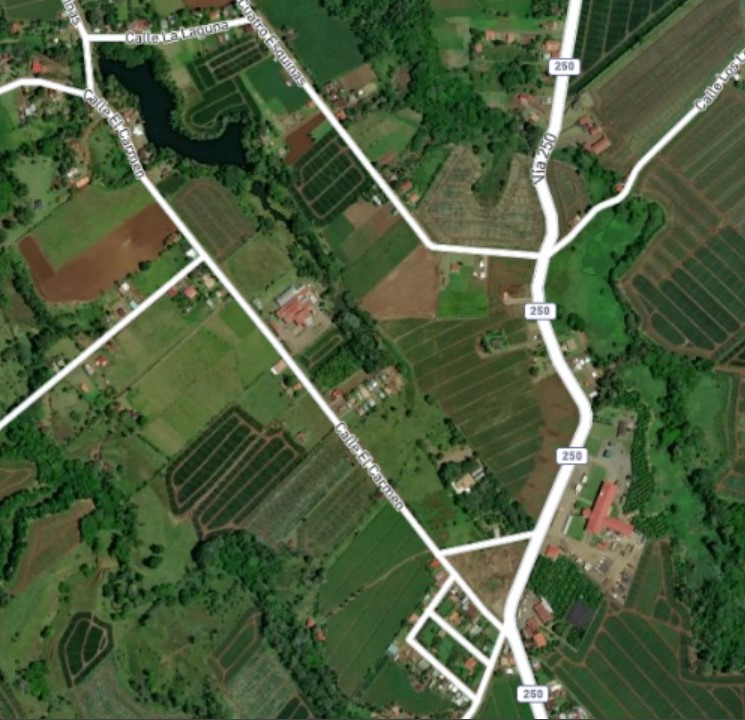
\includegraphics[width=\textwidth]{fig/satelliteZoom.jpg}
\caption{Satellite image corresponding to the polygon surroundings. \textit{Source: terrascope.be}}    
\end{subfigure}
\end{figure}


\begin{figure}[!ht]
\caption[PAL fields centroids and nearest nodes]{PAL fields centroids and nearest nodes. Centroids are coloured blue, and their nearest nodes are coloured red.}  
\label{allNodesPAL}
\centering
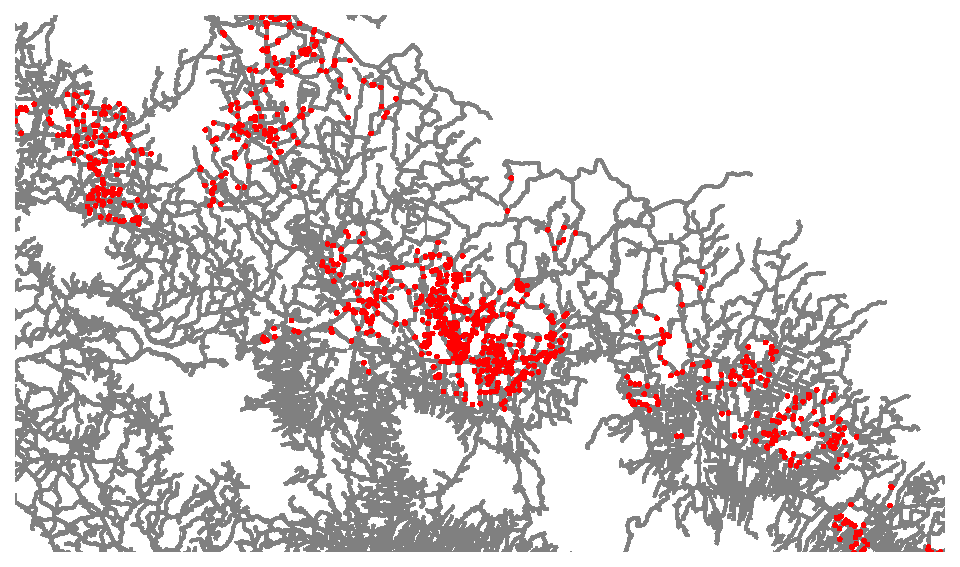
\includegraphics[width = \textwidth]{fig/allNodesNet.pdf}
\end{figure}


\subsection{Processing costs}
\label{costsch4}
The capacity of the facilities, $q_i$, and the costs of setting up a new facility, $f_i$, are estimated using the following data. As mentioned above, we estimate a supply of 4,836,731.25 tonnes of biomass (PAL) per year. Agricultural biogas plants usually have between 100 and 300 kW of power capacity, while industrial units exceed 1,000 kW. For the optimisation, we estimate costs based on 1,000 kW (1 MW) plants due to the important role economies of scale can play \citep{walla2008optimal, pinas2019economic}. Working at full capacity and with a power factor of 0.8, a 1 MW plant can generate 8,760 MWh per year $(0.8 \cdot 1 \si{\MW} \cdot 24 \si{\hour} \cdot 365 \si{\day})$. Assuming that each \si{\meter\cubed} of biogas generates approximately 2 kWh of useable electricity \citep{uddin2016biogas,suhartini2019estimation,swedishBio}, each plant must produce 4,380,000 \si{\meter\cubed} of biogas per year. With a conversion of 25.7 \si{\meter\cubed} per tonne of PAL \citep{arce2014determinacion}, each facility would require 170,428 tonnes (1050 hectares) of PAL each year, or 467 tonnes (3 hectares) every day. 

Capital and operating costs for a biogas plant depend on many factors, and empirical data are not available for the type of plant described in this study. Therefore, for the type of process described above, we provide an estimated range based on an extrapolation from a 250 kW, 137 \si{\tonne \per \day} biogas plant built in 2012 in Costa Rica \citep{sigmaanalysis}, average costs provided by the \citeauthor{ieaBio} and other sources \citep{salerno2017costs, obileke2022economic, newsGuatemala, newsSalvador, ICEbiogas, walla2008optimal}. We estimate that the economic lifespan of each biogas plant is 15 years, the capital costs to be between \$2 and \$4 million, and the annual operating costs to be between \$250 and \$450 thousand. \cref{biogasEstimates} depicts a summary of these estimates. 


\begin{table}[H]
\centering
\begin{threeparttable}
\caption{Estimates for the biogas plant in the optimisation}
\label{biogasEstimates}
\begin{tabular}{ll} 
\hline \hline  
Generator capacity          & 1 MW                      \\
Electricity generation      & 8,760 MWh/yr            \\
Biogas production           & 4,380,000 \si{\meter\cubed}/yr           \\
PAL processed               & 170,428 t/yr           \\
Capital costs               & \$2 to \$4 MM          \\
Operating costs             & \$250 to \$450 M/yr  \\
Facility lifespan           & 15 years                 \\ 
\hline   \hline     
\end{tabular}
\end{threeparttable}%
\end{table}


When deciding the available and suitable locations to place candidate facilities, the criteria present in the literature are varied and, on some occasions, arbitrarily defined. For example, \cite{jeong2019biodiesel}, who developed a supply chain optimisation model for camelina oil-derived biodiesel, selected county centroids as supply sites and also as candidate sites for the construction of new plants. \cite{caballero2007solving} selected candidate facility locations for residual processing plants based, for example, on unemployment rates and the centrality of the towns within the region. \cite{delivand2015optimal} implement well-defined criteria to select candidate facilities that consider planning rules, facility accessibility, and feedstock availability. We find the planning rules particularly relevant and useful when determining candidate facility locations.

Planning rules, also called zoning, are detailed rules on how a certain plot of land or area can be used. A famous example of zoning resolution is that of New York, adopted in 1916 to resolve the issue of property disputes about the height and size of buildings in business areas \citep{weiss1992skyscraper}. In Costa Rica, the zoning regulations are managed by the cantons \citep{planesRegCR}. According to the \citeauthor{PlanesReguladoresPortal}, 40 of the 82 cantons in the country have implemented a zoning regulation. However, most cantons do not publish spatial zoning maps showing which plots of land correspond to the different land uses, and only an official journal establishing the zoning regulations is publicly available. To our knowledge, only the San Carlos canton has developed a map of the zoning plan for the city of Quesada, as shown in \cref{sanCarlosPlan}.

\begin{figure}[!ht]
\caption[Zoning regulation applicable to the city of Quesada]{Zoning regulation applicable to the city of Quesada. Industrial zones are coloured green. \textit{Source: \citep{sancarlosPlan}}}  
\label{sanCarlosPlan}
\centering
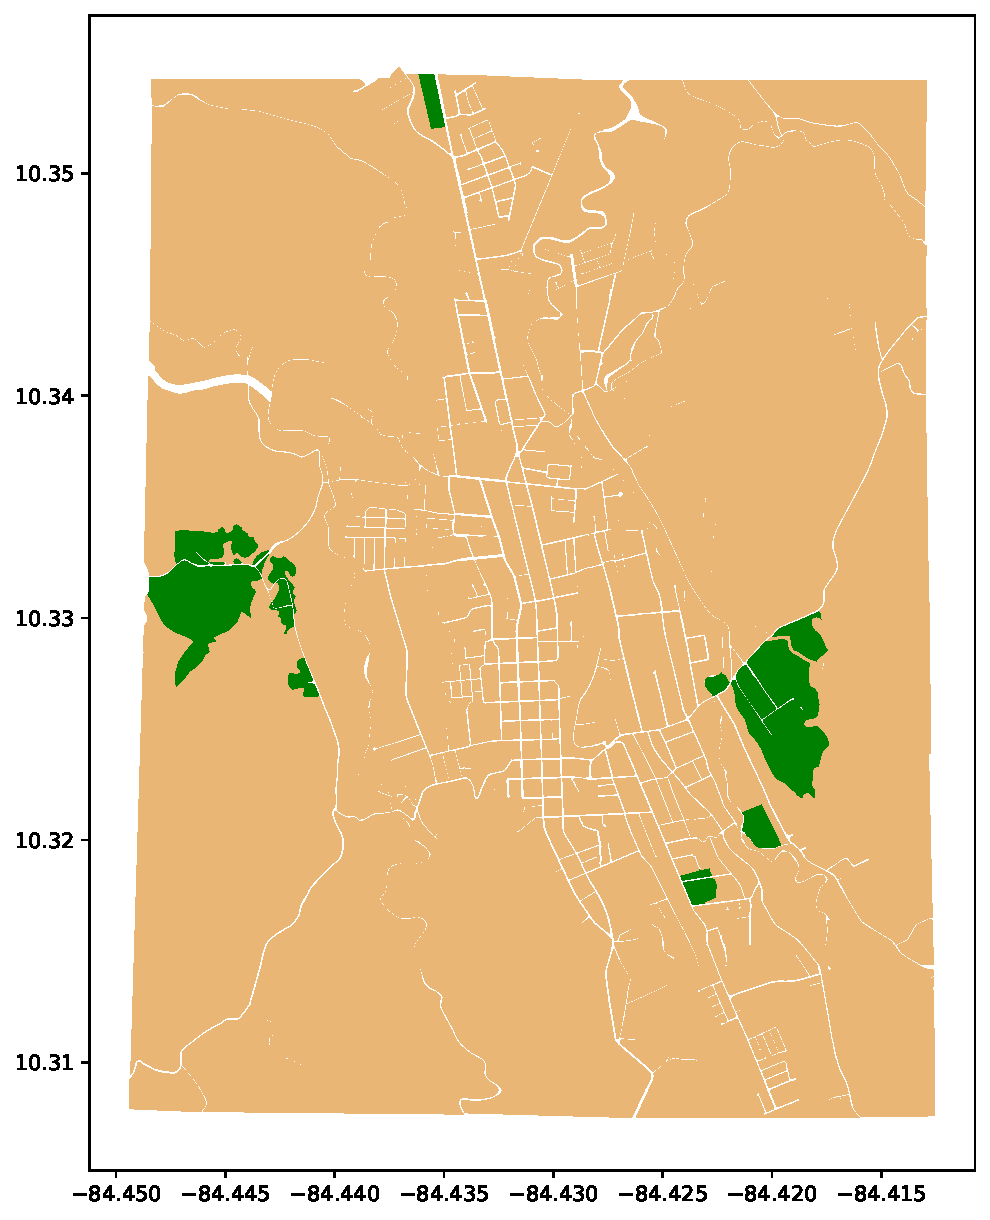
\includegraphics[width = 0.5\textwidth]{fig/sanCarlosPlan.pdf}
\end{figure}

In the case of the city of Quesada, defining potential processing facilities would be straightforward, as these are restricted to industrial zones. Since this type of data is not available for the rest of the country, it is not possible to implement criteria defined by zoning regulations in our FLP. Nevertheless, optimal locations determined by the algorithm can be used as a reference to locate the nearest available and suitable plots of land on a case-by-case basis. Following \citeauthor{delivand2015optimal}, we can at least restrict candidates to accessible locations using the country's road network to choose locations that are accessible by road and that do not fall within protected areas. Therefore, we generated 500 random candidate locations distributed along the street network inside the bounding box of the study area. The method of using network nodes as candidate facilities has been implemented before (e.g., see \cite{zhao2015does}). The generation of random nodes in the network, rather than generating an evenly spaced grid in (decimal) degrees, accounts for the geometry of the graph and guarantees uniform randomness \cite{boeing2017osmnx}. The candidates selected for the optimisation are shown in \cref{candidatesNet}. 

\begin{figure}[H]
\caption{Facility candidates randomly generated over the street network.}  
\label{candidatesNet}
\centering
\includegraphics[width=12cm]{fig/candidatesNet.pdf}
\end{figure}


\subsection{Transportation costs}

As with biogas plants, costs of transportation depend on many factors, and there are no easily accessible data. We estimate, based on several grey literature \citep{van2020cost, transportCost1, transportCost2}, a cost between \$0.20 and \$0.35 tonne-kilometre. We can also make an estimate by calculating the fuel price per kilometre. The fuel consumption of a typical Class 5, medium duty truck used to transport produce in Costa Rica (e.g., Isuzu N-Series with a load capacity of 7-9 tonnes), which is the range of 25-30 \si{l/100~km}. The price of fuel is currently \Colon750 (\$ 1.40) \si{\per \L} \citep{PreciosHistricosRECOPE}. This translates to a fuel cost of \$0.35 \si{\per \km}. This cost does not include any of the other transport-associated costs, such as fixed (e.g., investment costs, insurance) and variable costs (e.g., maintenance), staff costs, and operating costs. Thus, we believe that the estimate of \$0.20 - \$0.35 tonne-kilometre to be plausible. Finally, we should note that we do not consider chargeable weight (1 \si{\meter \cubed} = 333 \si{\kilogram} for road transport) a problem since the proposed solution implies shredding the PAL at the farm, which reduces the volume to a manageable level. The transport costs, $c_{ij}$, are then determined by: 

\begin{equation}
    c_{ij} = p_{tkm} \cdot \sum_{\substack{{i \in U} \\ j \in V}} k_{ij} \ d_j
\end{equation},

where $p_{tkm}$ is the cost per tonne-kilometre and $k_{ij}$ is the distance from the farm $j$ to the facility $i$.

Although it is common in location problems to use the Euclidean distance to calculate distances, the difference between using the road distance and the Euclidean distance is high in some cases \citep{pittayarugsarit2019comparison}. For this reason, we decided to calculate road distances by using the edges of the road network. 

\section{Results}

For the baseline results, we set the facility set-up costs to 3 MM (for a 15 years plant) and the annual operating costs to 350 M. Transportation costs were set at 0.275 tkm. The results obtained from the model consist of the number (30) and locations of biogas plant facilities, and the flows of biomass (PAL) supply from pineapple fields to the facilities. The total cost of the optimal solution is \$30,083,928, from which 16.5 MM are attributed to biogas facilities and 13,6 MM are attributed to transportation. This solution implies processing all the biomass (PAL), 4.9 MM tonnes, produced in the country each year. A map showing the optimal facilities location distribution is depicted in \cref{solutionMAP}. Due to the uncertainty of costs of both facilities and transportation, we analyse the effects of changes in set-up costs and transportation costs and show the different scenarios in the following section. The exact location and the set of facility-field combinations are provided in a CSV file. The MIP model was programmed in Python and solved using the Gurobi Optimiser version 10.0.1. More details can be found in \cref{suplmaterial}. 

\begin{figure}[!ht]
\caption[Spatial representation of the optimal solution for the FLP]{Spatial representation of the optimal solution for the FLP of biogas plants in Costa Rica}
\label{solutionMAP}
\centering
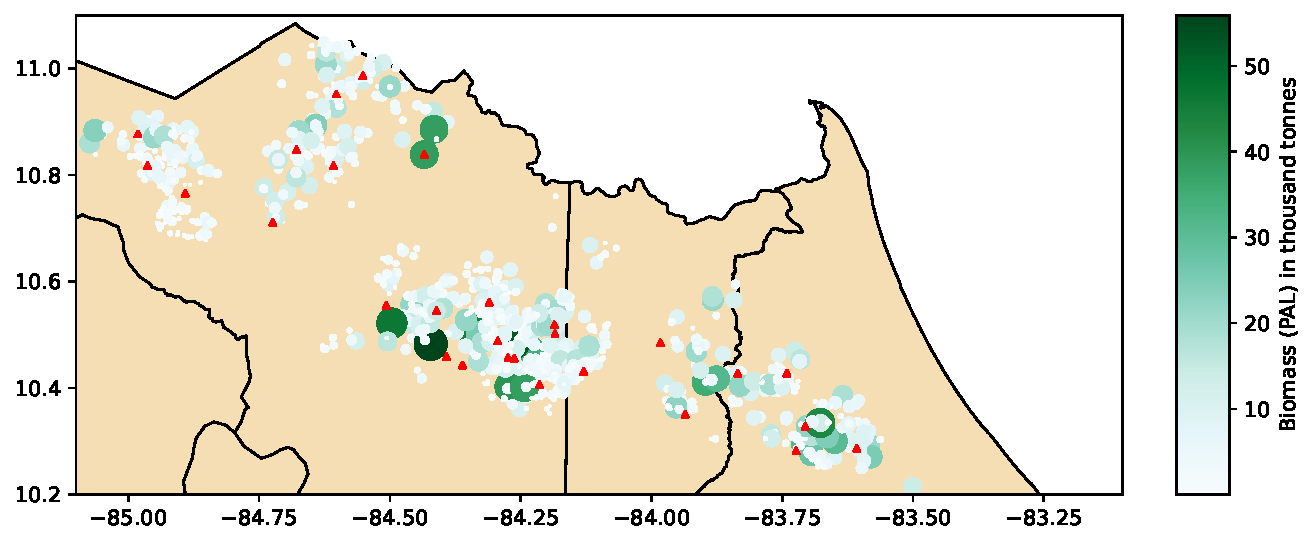
\includegraphics[width=\textwidth]{fig/resultsALL.pdf}
\end{figure}


\subsection{Sensitivity analysis}

We analyse the effect of different cost scenarios on the optimal number of locations. Since the facilities have a maximum capacity, there is a minimum number required to accommodate the entire supply of PAL. As can be seen in \cref{scenarioFLP}, the number of facilities varies depending on the different costs associated with transportation and facility setup. In scenarios with high transportation costs and small facility set-up costs, more facilities are open to minimise distances and costs of transportation. The number of facilities ranges between 28 and 34 and the total cost is between 24.5 and 38.3 MM. 

\begin{table}[H]
\centering
\begin{threeparttable}
\caption[Scenarios for the FLP problem]{Scenarios for the FLP problem. Total annual costs (MM) \& Number of Facilities in parentheses.}
\label{scenarioFLP}
\begin{tabular}{ccccc} 
\hline \hline  
&   & \multicolumn{3}{l}{Transport costs (tkm)} \\
%
&   & 0.20            & 0.275        & 0.35       \\
\multirow{3}{*}{\begin{tabular}[c]{@{}c@{}}Facility set-up\\ costs in \$ MM\end{tabular}}  
& 2 &  (24.5; 28)   &   (28.3; 30)  &  (34.9; 34)  \\
 & 3 & (26.2; 28)   &   (30.1; 30)  &  (36.5; 28)  \\
 & 4 & (28.0; 28)   &   (31.9; 28)  &  (38.3; 28)   \\
\hline   \hline     
\end{tabular}
\end{threeparttable}%
\end{table}


\section{Discussion}

Once the capacity of the plants has been decided, it is trivial to determine the minimum number of facilities needed to process the available PAL in Costa Rica. More interesting is to see how distances and, consequently, the costs of transportation affect the optimal number of facilities in the optimum. In this sense, the location of the supply points is the most important factor in our capacitated FLP problem. In the scenarios with more, less-supplied facilities, the total cost is probably overestimated because the set-up costs are considered for a 1 MW facility, which in such scenarios would not be needed. Nevertheless, the difference should be relatively small considering the small range in the number of opened facilities and the economies of scale attributed to their construction.

The total costs of the FLP, although based on estimates, provide us with a useful visualisation of the benefits an applied solution might bring. If we consider that the total cost to manage the stubble in the field (at least \$1000 per hectare \cite{hernandez2018impacto}) is similar to the average cost shown in \cref{scenarioFLP}, the valorisation of PAL through biogas production does not imply a larger investment in the long term. Additionally, if we consider that the 250,000 MWh of electricity generated from the facilities provide revenues of around \$30 MM (electricity is currently sold at \$0.12 (\Colon66.37) per kWh \cite{icePrices2023}) and that the extraction of PAL from the fields allows for faster pineapple production cycles, the valorisation scenario becomes economically reasonable and attractive. Finally, environmental costs should be considered. 

The simplicity of our model allows for new data to be incorporated easily and we expect the model to help in the decision-making process should facilities be built. In this sense, it is relevant to note that, by designing the type of solution described here, we idealise a collective and total solution which takes care of all the supply of PAL in Costa Rica. If pineapple producers were to implement this arrangement, partnerships would be needed to find a cost-effective solution. Considering that cooperatives are common in the pineapple industry, we consider this arrangement plausible. Another scenario we consider is that of an external company setting up a supply chain to collect, transport, and process the PAL. In such a case, an arrangement similar to that of municipal solid waste can be considered, with benefits for both pineapple producers and biogas producers.

The FLP has many variants, allowing for the modelling of different situations with different objective functions and constraints. The simple model shown here provides a solution for a tailored capacitated, multi-facility problem. Ideally, the model would optimise not only the number and location of a given type of capacitated facility but also the optimal capacity of the facilities accounting for economies of scale, i.e., for the different costs associated with processing one extra tonne of PAL in a facility with given fixed and variable costs. Two examples of this type of FLP can be found in \cite{wetterlund2012optimal, nordin2022optimal}. This type of FLP can provide more precise solutions which might involve building facilities of different sizes throughout the network, and its implementation is recommended.

\subsection{Extension of the model}

Cost minimisation is at the core of any operational challenge a company might face. FLP is a useful tool for stakeholders to consider options before making large, long-term investments. As exemplified in \cref{FLPlit}, FLP has expanded to incorporate environmental costs. When there is more than one objective to minimise, the FLP becomes a multi-objective MIP, which increases the complexity of the optimisation. The formulation of an environmental costs minimisation function is analogous to the economic costs minimisation function:

\begin{equation}
\label{envObjFun}
    \text{Min} \sum_{i \in U} \sum_{j \in V} e\_t_{ij} \ e\_f_{ij} + \sum _i \ y_i,
\end{equation} 

subject to the same constraints as \cref{objectivefun}, and where $e\_t_{ij}$ are the environmental impacts (usually measured in $CO_2$ emissions emitted) from transport between farm $j$ and the facility $i$, and $e\_f_{ij}$ are the environmental impacts associated with setting up and operating facility $i$. Similar to the operational costs function, the objective is to find the best number and location of facilities that minimise the total environmental impact of transportation and facilities. The complexity of the problem arises due to the nature of multi-objective MIPs, where the solution is expressed as a set of Pareto optima that represent the optimal trade-offs between the minimisation objectives. Since no single solution can be found, the challenge is to identify the preferable Pareto solution from the set based on given criteria and analysis of decision-makers \cite{limleamthong2018combined}. Usually, the Pareto frontier is shaped such that a solution with relatively low environmental impact can be chosen before the curve steepens towards relatively high economic costs. At that point, the gains from taking more environmentally friendly solutions are small compared to the very high economic costs \cite{harris2009multi}.

Biogas production, especially with second-generation feedstock such as PAL, has environmental benefits in terms of global warming potential and resource consumption compared to energy supply from fossil fuels. Furthermore, the environmental impacts of the construction and demolition of a biogas plant are relatively small, especially if a high utilisation ratio (long service life) of the plant is achieved \citep{hijazi2016review}. Thus, since the emissions from transportation can become significantly large, we expect the inclusion of environmental costs in the analysis to produce scenarios with a greater number of less-capacitated facilities. It is recommended to explore and implement a multi-objective FLP that accounts for both operational and environmental costs if a truly sustainable solution is to be obtained. 

\section{Conclusion}

The third set of research questions laid out in \cref{researchQ} has been answered throughout this chapter. The suitable locations and optimal spatial distribution of PAL processing plants were identified using the FLP making some simplifying assumptions about a potential real-case scenario. Deciding whether the processing of PAL should be centralised or decentralised depends on the type of valorisation process that is implemented. In the case of biogas production, a decentralised solution is more suitable for the case of Costa Rica considering the spatial distribution of pineapple fields in the country and the biomass processing capacity of biogas plants. The average scenario implies the construction of 30 biogas plants with a total annual cost of \$30.1 MM. Moreover, the results inform how the implementation of a biogas production scenario can provide operational cost savings to the pineapple industry in Costa Rica. 

Taking into account the uncertainty surrounding possible PAL valorisation solutions in Costa Rica, this study provides an optimistic initial step toward the implementation of a large-scale valorisation process. Should different types of valorisation techniques be considered, either as an alternative or an addition, this model provides the tools to analyse the most cost-effective operational solution. Since several value-added goods can be produced with PAL, as described in \cref{neweconomy}, we contemplate the addition of other processes to the biogas production chain, e.g., fibre extraction from the leaves prior to anaerobic digestion. This cascading solution would take advantage of the supply chain to integrate processes and generate greater value. From the FLP design point of view, this might require modelling a multi-echelon problem which would account for the distribution of PAL-based products to demand points. 

The analysis produced here is limited by the available data and, thus, stringent assumptions and simplifications were made. As more data on the potential costs, capacity, and production of PAL-fed biogas plants are known, more accurate results from the model will be obtained. Furthermore, the potential locations of the facility used in the analysis were randomly selected from the network nodes. This ensures connectivity in the network but does not consider regulations related to zoning or land availability. A true solution will be close to the one provided in the study, but these considerations must be taken into account. Finally, we recognise the importance of accounting for environmental impacts when finding FLP solutions, as these might change the number and spatial arrangement of facilities considerably. Estimating such impacts can also shed light on the environmental costs of valorising PAL compared to managing it in the field with agrochemicals and burning. Since PAL is a second-generation feedstock and does not compete with other crops or land use, we expect the costs to be relatively low.

